% Chapter 2 (probably)
% STTs

\chapter{Stratosphere to Troposphere Transport of ozone} % Main chapter title
\label{ch_o3}

%----------------------------------------------------------------------------------------
%	Ozone Section
% 	TODO:SOME PORTION OF THIS SHOULD BE IN INTRO, to be worked out much later
%----------------------------------------------------------------------------------------
\section{Background}
  \label{ch_o3:sec:ozone}

  \subsection{Historical estimates}
    Tropospheric ozone is important for both air quality and climate change. 
    The impact of stratospheric ozone on the troposphere is dependent on weather, season, temperature, and many other factors. 
    For example changing ozone in the tropical tropopause layer by 5\% causes 0.5 K dec$^{-1}$ radiative heating \citep{Forster2007}.
    In Australia, records of ozone profiles provided by the Department of the Environment can be used to determine how often stratospheric ozone descends into the troposphere.
    

    Over the industrial period, tropospheric ozone, which is the third most potent greenhouse gas, has been estimated to exert a radiative forcing equivalent to a quarter of the CO2 forcing. 
    Ozone is present in the troposphere due to a variety of dynamical and photochemical processes, including downward  transport from the ozone-rich stratosphere and anthropogenic pollution.
    The primary sources of tropospheric ozone are chemical creation and stratospheric input, estimated using a model ensemble to be $5100\pm600$ Tg/yr and $550\pm170$ Tg/yr, respectively \citep{Stevenson2006}.
    The primary sinks are chemical destruction and dry deposition, estimated to be $4700\pm700$ Tg/yr and $1000\pm200$ Tg/yr, respectively \citep{Stevenson2006}.

  \subsection{Tropospheric production}
  
    Ozone is a toxic trace gas which increases mortality rates when populations are exposed for extended periods of time.
    The amount of global premature deaths per year due to atmospheric ozone exposure has recently been estimated at $\sim$150-470 thousand \citep{Silva_2013, Lelieveld_2015}.
    Long term effects of ozone overexposure increase the risk of respiratory disease and may also increase other cardiopulmonary risks \citep{Jerrett_2009}.

    The Ambient Air Quality (AAQ) National Environment Protection Measure (NEPM), which is the Australian framework for air quality measurement and reporting aiming for ``adequate protection of human health and well-being'' has set national standards and benchmarks for reporting. The NEPM covers six chemical groups including Ozone (O$_3$), and the benchmarks are shown in figure \ref{ch1:fig:nepm}.

    \begin{figure}[!htbp]
      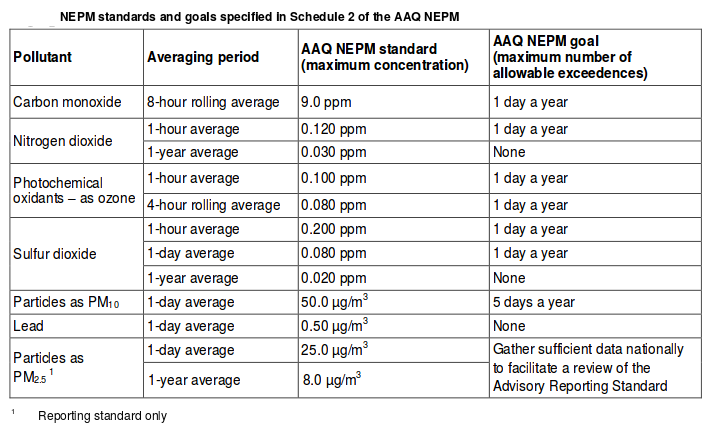
\includegraphics[width=\textwidth]{Figures/NEPMStandards.png}
      \caption{ NEPM standards taken from National Environment Protection Council annual report 2012-2013 \citep{nepc_annuals}. }
      \label{ch1:fig:nepm}
    \end{figure}
    
    The primary source of ozone in the lower troposphere is chemical formation following emissions of precursor gases, including VOCs, and NO$_X$.
    Globally the greatest sources of NO$_X$ include fossil fuel combustion ($\sim$50\%), biomass burning ($\sim$20\%), lightning, and microbial activity in soils \citep{Delmas_1997}.
    Estimates using CHASER (a global Chemical Transport Model (CTM)) constrained by measurements from two satellites as well as the in-situ measurements taken through LIDAR and aircraft (INTEX-B) put global tropospheric NO$_X$ emissions at 45.4 TgN yr$^{-1}$ in 2005 \citep{Miyazaki2011}.

    The majority of this chemical formation is due to photochemical oxidation of carbon monoxide (CO), methane (CH$_4$), and other Volatile Organic Chemicals (VOCs) in the presence of nitrogen oxides (NO$_X$ $\equiv$ NO $+$ NO$_2$) \citep{Stevenson2006}.

    Photolysis of NO$_2$ forms NO + O(3P), which combines with O$_2$ to form O$_3$, leading to reaction with NO to form NO$_2$ + O$_2$.
    These reactions reach a steady state where O$_3$ is proportional to the ratio between NO$_2$ and NO \citep{Sillman_2002}.
    The following formulae show an example of this with CO, however, similar reactions occur for many VOCs:
    \begin{eqnarray*}
      NO_2 + hv &\overset{k_1}{\rightarrow}& NO + O({}^3 P) \\
      O({}^3 P) + O_2 &\overset{M}{\rightarrow}& O_3 \\
      NO + O_3 &\overset{k_2}{\rightarrow}& NO_2 + O_2 \\
      \left[O_3\right] &\sim& \frac{k_1}{k_2} \frac{\left[NO_2\right]}{\left[NO\right]} \\
      OH + CO &{\rightarrow}& HOCO \\
      HOCO + O_2 &{\rightarrow}& HO_2 + CO_2 \\
      HO_2 + NO &{\rightarrow}& OH + NO_2 \\
    \end{eqnarray*}
    where $k_1$ and $k_2$ are reaction rates, and hv represents photons.
    The balance of these reactions is:
    \begin{eqnarray*} CO + 2O_2 + hv {\rightarrow} CO_2 + O_3 \end{eqnarray*}
    Note that this reaction pathway only occurs during the day.

    Isoprene (C$_5$H$_8$) is a precursor to ozone through radical oxidative chemistry. Isoprene in the atmosphere reacts rapidly with hydroxyl radicals (OH) and then O$_2$ to form peroxy radicals (RO$_2$).
    These react with nitrogen oxides and can lead to ground-level ozone formation similarly to the CO reaction listed prior.

    Formaldehyde (HCHO) together with NO$_2$ regulate tropospheric oxidation capacity through O$_3$ production, as well as being health hazards.
    The HCHO/NO$_2$ ratio can be used to determine whether surface O$_3$ is NO$_2$ or VOC limited \citep{Mahajan2015}.
    If O$_3$ is NO$_2$ limited then an increase in NO$_2$ will increase O$_3$ levels while an increase in HCHO will not, and vice versa when O$_3$ is HCHO limited.
    NO$_2$ is a common pollutant in populated areas, released primarily by combustion in power generation and transport. 
    Outside of cities in Australia, VOCs and NOx are emitted from biogenic sources, although lightning, and biomass burning (most clearly in the Northern Territory) also play a role \citep{Guenther2006, VanDerA2008}.

  \subsection{Stratosphere to Troposphere ozone Transport (STT)}
  
    While the amount of tropospheric ozone is small compared with that found in the stratosphere, it is an important constituent.
    Ozone-rich air mixes irreversibly down from the stratosphere during meteorologically conducive conditions \citep{Sprenger2003,Mihalikova2012}; these are referred to as Statosphere - Troposphere Transport events (STTs). 
    In the extra-tropics, STTs most commonly occur during synoptic-scale tropopause folds \citep{Sprenger2003} and are characterised by tongues of high Potential Vorticity (PV) air descending to low altitudes. 
    PV is a metric which can be used to determine whether a parcel of air is stratospheric, based on its local rotation and stratification.
    Within the troposphere PV values are typically low, increasing rapidly into the stratosphere due to the increased static stability.
    
    These ozone rich tongues become elongated and filaments separate from the tongue which mix into tropospheric air.
    Stratospheric ozone brought deeper (lower) into the troposphere is more likely to affect the surface ozone budget and tropospheric chemistry \citep{Zanis2003,Langford_2009}.
    A high correlation is found between lower stratospheric and tropospheric ozone \citep{Terao2008} with the highest STT associated with the jet-streams over the oceans in winter.
    Irreversible STT of ozone is important for explaining tropospheric ozone variability \citep{Tang2010}.
    Stratosphere to Troposphere ozone transport can potentially increase regional surface ozone levels above safe levels \citep{Zhang2014}.
    
    While photochemical production is the dominant source, stratosphere to troposphere transport of ozone is also important and climate change may drastically increase this quantity \citep{Hegglin_2009}.
    In a future climate, a warmer, wetter troposphere will change the chemical processing of ozone.
    Dynamical processes such as STT, boundary layer ventilation and convection changes will alter tropospheric ozone distributions.
    \citet{Hegglin_2009} estimate that climate change will lead to increased STT of the order of 30 (121) Tg yr$^{-1}$ relative to 1965 in the southern (northern) hemisphere due to an acceleration in the Brewer Dobson circulation. 
    
    STT events are characterised in the ozonesondes' vertical profiles of ozone as altitudes in the troposphere where the ozone mixing ratio exceeds a specified threshold. 
    Usually stratospheric ozone mixes irreversibly down into the troposphere in a synoptic-scale tongue of air: the vertical ozone profile observed by the ozonesonde depends upon the time in this cycle that it is observed \citep{Sprenger2003}. 
    As such, the altitude of the tropospheric ozone peak due to an STT event, and the amplitude of the event above the background tropospheric ozone profile, vary in space and time.

%----------------------------------------------------------------------------------------
%	Ozone Sondes
%----------------------------------------------------------------------------------------

\section{Instruments and data sets}
  \subsection{Atmospheric Infrared Sounder (AIRS)}
    AIRS is an instrument on board NASA's AQUA satellite, which overpasses the globe roughly daily on a sun-synchronous orbit gathering measurments at 1:30pm local time.
    AIRS is a high spectral resolution spectrometer with 2378 bands in the thermal infrared (3.7 - 15.4 $\mu$m) and 4 bands in the visible (0.4 - 1.0 $\mu$m).
    One of the products shared by NASA is total column carbon monoxide (AIRS3STD \citep{AIRS3STD}).
    Using this product to exclude possible fire plume transport from STT analysis is done in section \ref{ch_o3:sec:airs_fire_filter}.
  
  \subsection{Sondes}
  
    Ozonesondes are weather balloons with an attached instrument which measures ozone concentrations roughly every 100m up to around 30km. These ozonesondes provide a high-vertical resolution profile of ozone.
    
    In this work sonde data from three sites are utilised: Davis (lat, lon, UTC~$+7$), Macquarie Island (lat, lon, UTC~$+11$), and Melbourne (lat, lon, UTC~$+11$).
    Ozonesondes are launched approximately weekly from these three sites, we exame data from up to 2013, starting in 2004 at Melbourne and Macquarie Island, and 2006 at Davis.
    More frequent ozonesonde launches occur at Davis during the spring ozone hole season than at other times of the year \citep{Alexander2013}.
  
  \subsection{European Centre for Medium-Range Weather Forecasts (ECMWF) Re-Analysis - Interim data set (ERA-I)}
    Ozonesondes provide much higher vertical resolution profiles of ozone than that available from reanalyses products.
    The downside is that one data point per week from an ozonesonde release is too low to be in itself useful to diagnose the evolution of STT exchange over time-scales associated with normal synoptic scale weather patterns present in the extra-tropics.
    The ECMWF provides a useful meteorological model based on assimilated data.
    Here, ozonesonde data are supplemented with the ERA-I dataset \citep{Dee2011} to enable construction of an STT exchange climatology.
    The dataset is called a re-analysis due to the fact that the whole timeline gets re-run when the climatological model is updated.
    This provides uniform data output over a long time period.
    
    The ERA-I data we used for synoptic weather was of one degree horizontal resolution with pressure levels at 200, 300, 400, and 500 hPa.
    For individual cases ERA-I data was downloaded at .25 degree horizontal resolution with the full 34 pressure levels from 1000 to 1 hPa.
    Note that 34 levels up to the top of the atmosphere is not enough to determine vertical transport when considering only a single vertical profile, however a precise view of coincident weather can determine probable cause of ozone flux.
    

%----------------------------------------------------------------------------------------
%	STT Detection Method
%----------------------------------------------------------------------------------------
\section{STT Detection}

  \subsection{Aim}
    Using several years of ozonesonde flights from three locations spanning the latitudes of the Southern Ocean, we create and examine a quantitative method for detecting ozone STT events from ozone vertical profiles.
    With a quantitative method of STT detection characterisation of the seasonal cycle of STT events and determination of their contribution to the total amount of tropospheric ozone is possible.
    Examination of the ozone intrusions and case studies allows us to relate these STT to meteorological events.
    Finally we use the same filtered sonde data in order to extract a lower bound estimate of how much of the tropospheric column ozone is due to STT events.

  \subsection{Tropopause Heights}
    Two definitions of the tropopause height are calculated: the standard lapse rate tropopause \citep{WMO1957}, and the ozone tropopause \citep{Bethan1996}.
    At Davis, the ozone tropopause defintion is modified for polar sites, following \citet{Tomikawa2009,Alexander2013}. 
    While the ozone tropopause can be less robust during stratosphere-troposphere exchange, it performs better than the lapse rate tropopause at polar latitudes in winter and near jet streams in the lower stratosphere \citep{Bethan1996}. The lower of these two tropopause altitude-definitions is referred to as the tropopause for this study.
    This choice of the lowest altitude of the tropopause avoids occasional unrealistically high tropopause heights due to perturbed ozone or temperature measurements.

    The monthly mean tropopause altitudes at each location are shown in Figure~\ref{ch_o3:fig:seasonaltpheights}, along with the subset of altitudes from profiles for which an STT event was determined. 
    The seasonal cycle in tropopause altitude at Melbourne is clearly apparent, as is the decreasing tropopause altitude poleward. 
    Seasonally averaged ozone as recorded over the three stations (Figure \ref{ch_o3:fig:seasonaltropozone}) shows increased ozone extending down through the stratosphere during the peak STT months over Melbourne.
    It is worth noting that tropopause altitudes at Davis may exceed 11~km altitude under certain synoptic conditions \citep{Alexander2013}: the relation of tropopause altitude with individual STT events will be investigated in detail below.

    \begin{figure}\begin{center}
      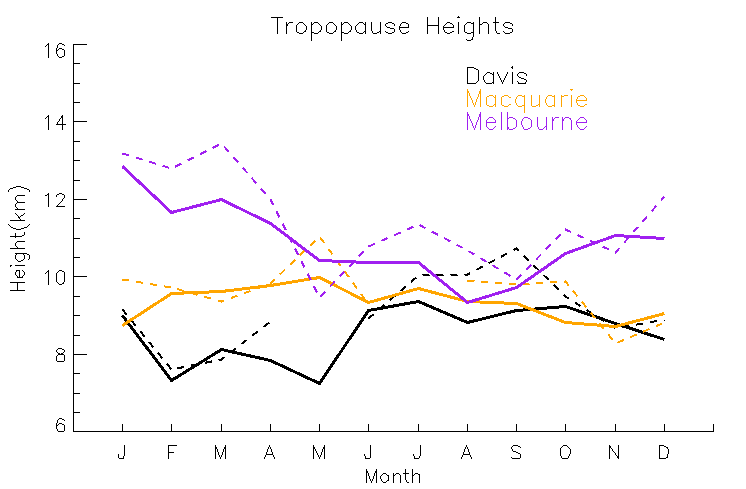
\includegraphics[width=0.8\columnwidth]{Figures/Ozone/tpheights}
      \caption{
	Monthly mean tropopause altitudes (minimum of lapse-rate and ozone defined tropopauses). Dashed lines show 'event only' seasonal tropopause altitudes.%
      }
      \label{ch_o3:fig:seasonaltpheights}
    \end{center}\end{figure}

    \begin{figure}\begin{center}
      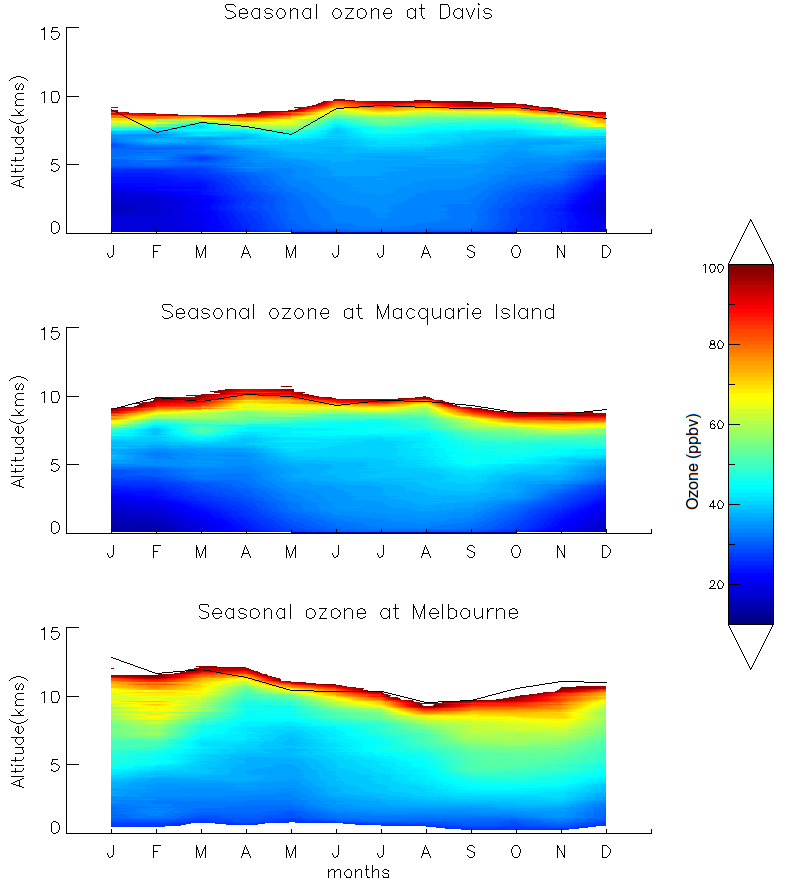
\includegraphics[width=0.8\columnwidth]{Figures/Ozone/seasonaltropozone}
      \caption{
	Seasonally averaged ozone over Davis, Macquarie, and Melbourne measured by ozonesondes.
	Black solid lines show seasonal tropopause heights.%
      }
      \label{ch_o3:fig:seasonaltropozone}
    \end{center}\end{figure}
    
  \subsection{Fourier bandwidth (or bandpass) Filtering}
    \label{ch_o3:sec:bandpassfilter}
    A Fourier bandwidth filter can remove components of a line based on the components frequency. 
    For example: a noisy ozone profile can be ’cleaned’ by removing the high frequency components, while growth of ozone with altitude in the profile can be removed as a low frequency component. 
    
    TODO: Add description, equation(s) and maybe a simple example plot here as well as limits of filter.
    The basic idea of a Fourier bandwidth filter is that any finite length function can be written as a series of trigonometric functions:
    \begin{equation} \label{ch_o3:eqn:FourierSeries}
      f(t) = \Sigma_i C_{w_i} \cos \left( w_i t - \theta_i \right)
    \end{equation}
    
    Once we split our function into specific frequencies ($w_i$) we can simply remove the terms which fall outside our desired wavelength range.
    One limitation is that the reconstructed function may be quite different at either end of the input range.
    
    In the continuous spatial domain, this is done is through taking the Fourier transform which can convert our function to a complex frequency domain:
    \begin{equation*}
      F(w) = \frac{1}{\sqrt{2\pi}}\int_{-\infty}^{\infty}{ f(t) e^{-iwt} \mathrm{d}t }
    \end{equation*}
    where t describes the spatial input range (in our case altitude).
    Then it's possible to remove the portion of the function outside the desired frequency before inverting the Fourier transform:
    \begin{equation*}
      f(t) = \frac{1}{\sqrt{2\pi}}\int_{-\infty}^{\infty}{ F(w) e^{iwt} \mathrm{d}w }
    \end{equation*}
    
    This whole process is slightly changed when we consider discrete dimensions as we must whenever solving numerically or handling real world resolved datasets.
    There is a ``shortcut'' method which 
    
    
  \subsection{Bandwidth filter applied to ozonesondes}
    
    With a Fourier bandwidth filter used on ozone profiles over Davis, Macquarie, and Melbourne we quantitatively determine instances of Stratosphere to Troposphere Transport events through the following method.
    The vertical profiles of ozone volume mixing ratio are linearly interpolated to a regular grid with 20m resolution up to 14km altitude and are then bandpass filtered so as to retain perturbations which have vertical scales between 0.5km - 5km. 
    The choice of band limits is set empirically, but we note that to define an STT event, a clear increase above the background ozone level is needed, and a vertical limit of $\sim 5$~km removes seasonal-scale effects. 
    The ozone perturbation profile is analysed at altitudes from 4~km above the surface (to avoid surface pollution events) and 1~km below the tropopause (to avoid the sharp transition to stratospheric air producing spurious false positives). 
    Perturbations above the 99~th percentile (locally) of all ozone levels are initially classified as STT events.
    
    In order to remove unclear 'near tropopause' anomalies we remove events where the gradient between the maximum ozone peak and the ozone at 1~km below the tropopause is greater than $-20$~ppbv~km$^{-1}$ and simultaneously require that the perturbation profile does not drop below zero between the event peak and the tropopause.
    The addition of these filters removes several events, each with an ozone peak which could not be definitively said to be seperated from the stratosphere.
    
    To provide a conservative estimate of ozone flux into the troposphere for each event, the ozone concentration is integrated vertically over the interval for which an STT event is identified.
    An example of an ozone profile is illustrated in Figure~\ref{ch_o3:fig:filterEG} and indicates how the algorithm detects an STT event, defines the event boundaries, and calculates the ozone flux.
    
    \begin{figure}[!htbp]
      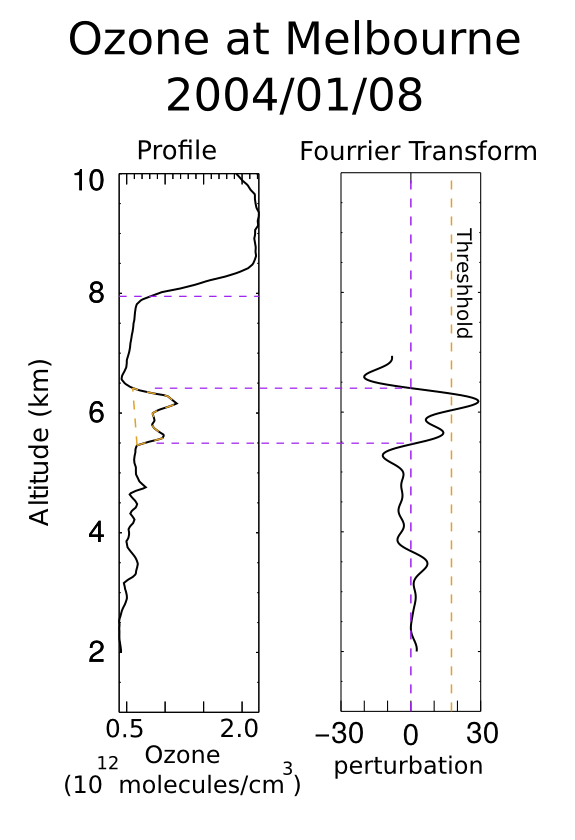
\includegraphics[width=\columnwidth]{Figures/Ozone/filtereg.png}
      \caption{ (a) An ozone profile between 2km altitude and the tropopause (indicated by the dashed vertical line).
      The 'flux' area shows the estimate of stratospheric impact on tropospheric ozone.
      (b) The 99th percentile of filtered ozone perturbations (green dashed line) and the technique for determining the vertical extent of the 'event' (red dashed and solid lines).%
      }
      \label{ch_o3:fig:filterEG}
    \end{figure}
    
  \subsection{Case Studies}
    We examine two STT case studies in detail to illustrate the synoptic scale conditions in which they can occur above Melbourne.

    A cut-off low pressure system passed over Melbourne on 3~February 2005 (Figure~\ref{ch_o3:fig:MelbourneCases}b).
    The ozonesonde profile indicated low lapse-rate and ozonesonde tropopauses (both $> 450$~hPa, see Figure~\ref{ch_o3:fig:MelbourneCases}a). 
    An ozone intrusion into the troposphere is identified by our detection algorithm at $\sim520$~hPa.

    STT events also occur during frontal passages, an example of which is illustrated in Figure~\ref{ch_o3:fig:MelbourneCases}d over south-eastern Australia.
    The tropopauses are much higher at this time and an ozone intrusion is identified centred around 200~hPa.
    Note the separation between this intrusion and the ozone tropopause (marked by the green dashed line), indicating the start of the stratosphere above Melbourne.
    During the frontal passage, stratospheric air descends and streamers of ozone-rich air likely break off and mix into the troposphere \citep{Sprenger2003}.
    TODO: talk about pvu lines here.

    The relative humidity profiles are anticorrelated with ozone in the upper troposphere for these events, indicating again the stratospheric origin of the ozone-rich air mass.
    TODO: show latlon plots for the sites and describe lowered tropopause in more detail here.
    Some of this stratospheric air gets mixed into the troposphere, with one ozonesonde column showing an intrusion at around 200 hPa, with dry ozone rich air peaking below the tropopause(Figure \ref{ch_o3:fig:MelbourneCases}c).
    
    \begin{figure}[!htbp]
      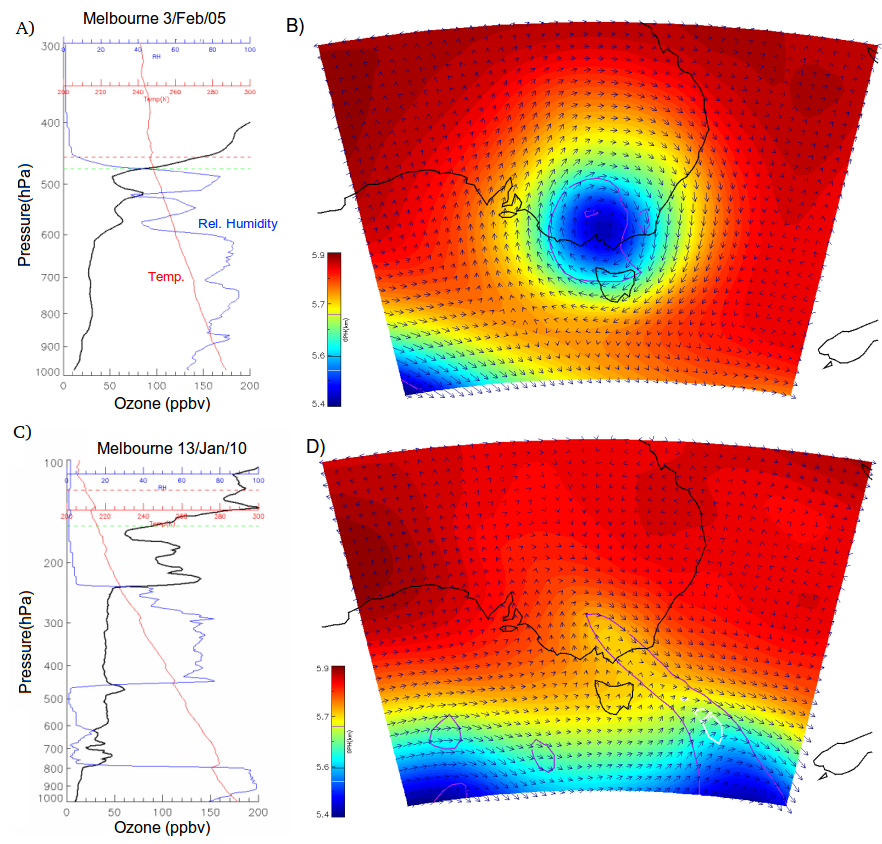
\includegraphics[width=\columnwidth]{Figures/Ozone/Cases}
      \caption{
	Vertical profiles show ozone ppbv (black line), relative humidity (blue line), and temperature (red line) for (a) 3~February 2005 and (c) 13~January 2010. Synoptic weather maps show the 500 hPa pressure level taken from the ERA-Interim reanalysis on (b) 3~February 2005 and (d) 13~January 2010. 
	Vectors show wind direction and speed while the colour indicates the geopotential height. 
	Also visible are the line contours of potential vorticity units, 1 PVU in purple and 2 PVU (often used to determine dynamical tropopause height) in white.}
      \label{ch_o3:fig:MelbourneCases}
    \end{figure}
    
  \subsection{Site summaries}
    Running the ozonesonde dataset through our bandpass filter and analysing the results allows an overview of the yearly cycle and event characteristics.
    These seasonal cycles and event characteristics for each of the three locations are presented in Figure~\ref{ch_o3:fig:SummaryMelbourne} to Figure~\ref{ch_o3:fig:SummaryDavis}.
    There is an annual cycle in the occurrence frequency of STT events (with a summertime peak) above Melbourne and Macquarie Island. However, the occurrence frequency of STT events above Davis is relatively constant throughout the year.

    The majority of events occur within 3~km of the tropopause at both Melbourne and Macquarie Island, and within 2~km of the tropopause at Davis. 
    STT event altitudes most commonly occur at 6 -- 10~km above Melbourne and below 8~km at Davis but are distributed more evenly in altitude at Macquarie Island. 
    
    \begin{figure}[!htbp]
      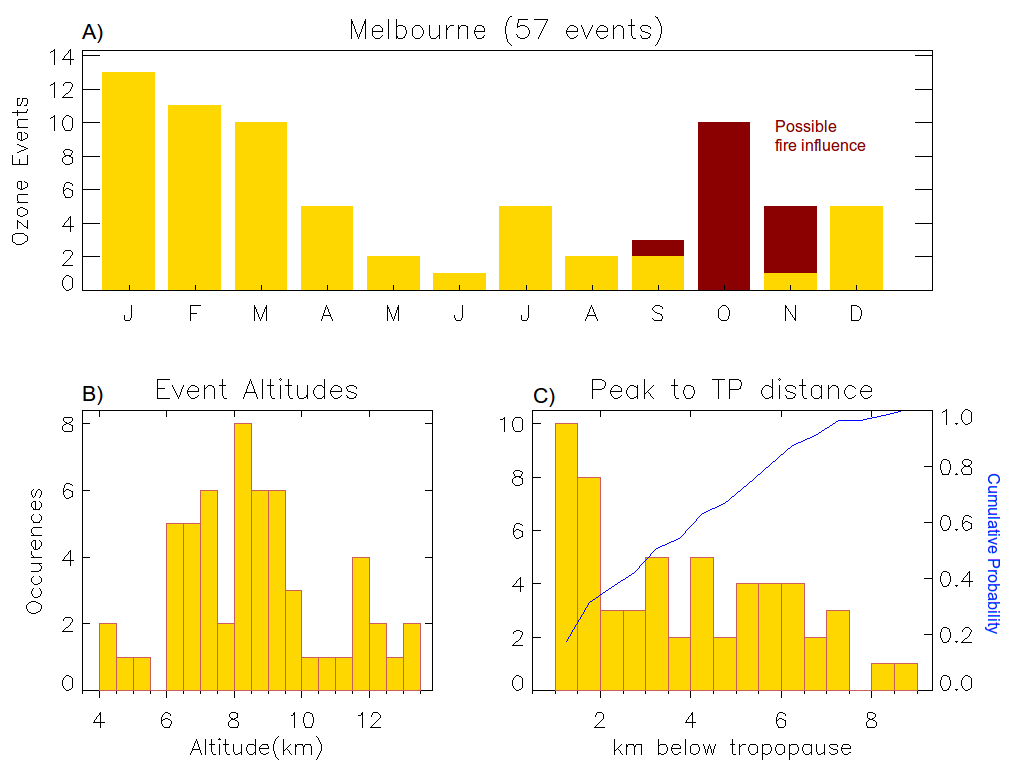
\includegraphics[width=0.8\columnwidth]{Figures/Ozone/Summary_Melb}
      \caption{
	The climatology of STT events at Melbourne: (A) Events sorted by month from the entire Melbourne ozonesonde dataset. The events filtered out as possibly smoke plume influenced are indicated in red. (B) The occurrence distribution of the ozone peak altitude. (C) The distance between the ozone peak and the tropopause (bars)  and the cumulative probability function of these distances (blue line).%
      }
      \label{ch_o3:fig:SummaryMelbourne}
    \end{figure}

    \begin{figure}[!htbp]
      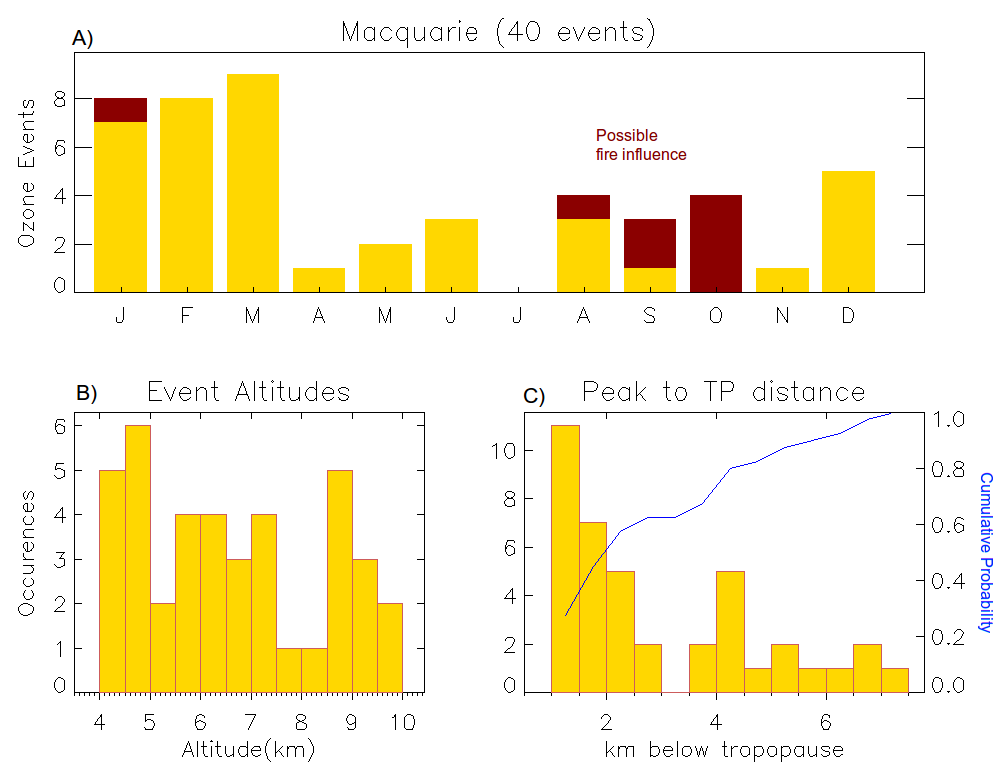
\includegraphics[width=0.8\columnwidth]{Figures/Ozone/Summary_Macq}
      \caption{
      As for Figure~\ref{ch_o3:fig:SummaryMelbourne} except showing the Macquarie Island STT events.%
      }
      \label{ch_o3:fig:SummaryMacquarie}
    \end{figure}

    \begin{figure}[!htbp]
      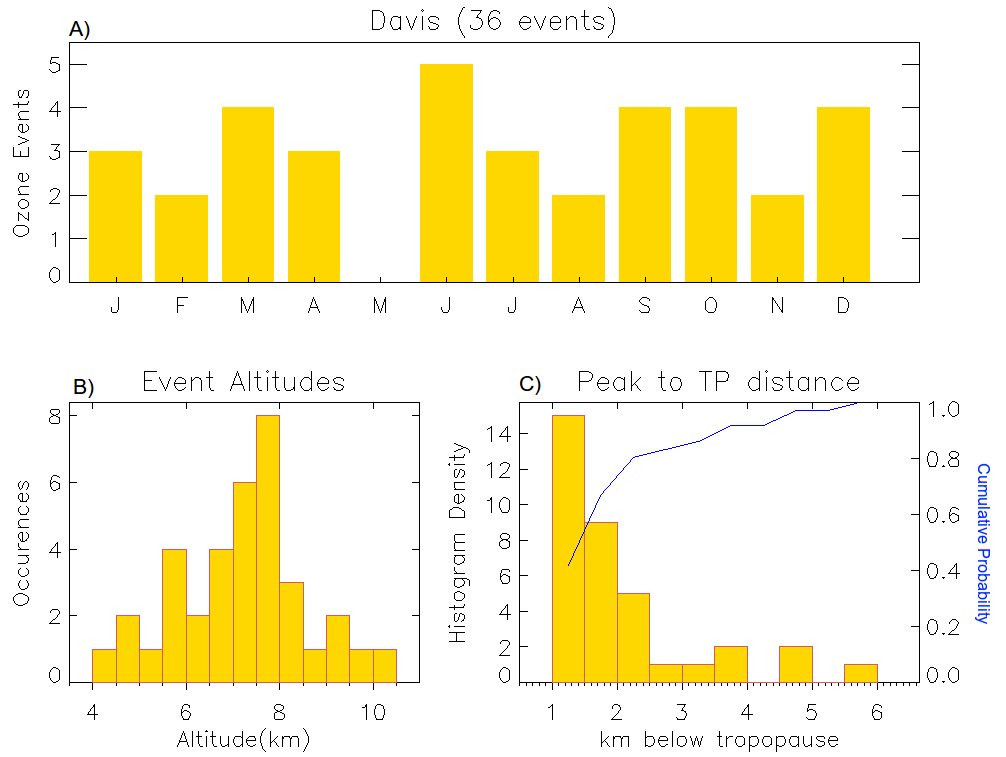
\includegraphics[width=0.8\columnwidth]{Figures/Ozone/Summary_Davi}
      \caption{
      As for Figure~\ref{ch_o3:fig:SummaryMelbourne} except showing the Davis STT events.%
      }
      \label{ch_o3:fig:SummaryDavis}
    \end{figure}
    
%----------------------------------------------------------------------------------------
%	STT impact determination method
%----------------------------------------------------------------------------------------
\section{Stratosphere to Troposphere flux analysis}
  \subsection{Determining a minimum estimate of stratospheric influence}
    Determining how much ozone is transported from the stratophere with only a two dimensional line vector of ozone concentrations is tricky. 
    It is possible to give a lower bound on stratospheric ozone influence by determining the ozone spike above a baseline amount for each column. 
    This is a lower bound as it ignores dispersed ozone and any secondary peaks which may also be due to stratospheric transport.
    
    Using our estimate of STT ozone flux (see section \ref{ch_o3:sec:bandpassfilter}) we find a lower bound for the STT ozone flux over each of our three sites, excluding possible fire influence.
    Figure \ref{ch_o3:fig:fluxsummary} shows the climatological mean fraction of total tropospheric column ozone attributed to stratospheric ozone intrusions at each site, on days when an STT event occurs. These flux amounts are calculated after removal of the biomass burning events, although leaving the burning events in changes the means by less than 5\%. The mean fractions of stratospheric ozone are 2--4\%, although the largest fractional ozone in the tropospheric column attributed to stratospheric air exceeds 10\% at all locations.
      

    \begin{figure}[!htbp]
      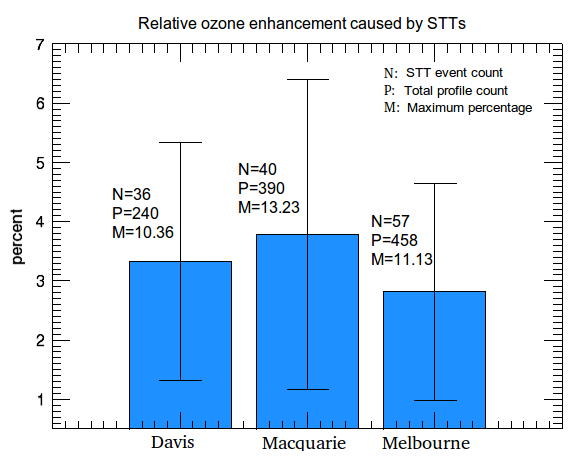
\includegraphics[width=0.8\columnwidth]{Figures/Ozone/FluxSummary_notrans.png}
      \caption{
      Fraction of total tropospheric column ozone attributed to stratospheric air intrusions during STT events. Error bars indicate one standard deviation.%
      }
      \label{ch_o3:fig:fluxsummary}
    \end{figure}
  

%----------------------------------------------------------------------------------------
%	NON-STT Influences
%----------------------------------------------------------------------------------------
\section{Non-STT influences on ozone at southern latitudes}

  \subsection{Fire Plumes}
    Ozone production due to fire smoke plumes is complex and affected by photochemistry, fuel nitrogen load, and atmospheric plume interactions both during transport and at the plume's destination. Ozone precursors include nitrogen oxides ($NO_x = NO + NO_2$) and non methane volatile organic compounds (NMVOCs). Large biomass burning events emit substantial ozone precursors, some of which are capable of being transported far from their origins. NO$_x$ can be transported far downwind due to peroxyacetyl nitrate (PAN) thermal decomposition and this can lead to enhanced ozone far from the source of a fire \citep{Jaffe_2012}.
    
    \citet{Pak2003} show a tropospheric ozone spike over SE Australia in September and using back trajectories suggest that the air masses over Melbourne on this day also passed over South Africa and the higher altitude air also passed through South America.
    The Australian fire season spans most of the year, sweeping southwards as shown in figure and may occasionally affect the ozone columns above either of Macquarie and Melbourne. However, the influence from regional burning is unlikely to affect the ozone concentration above 4~km altitude and most of the smoke from the northern half of Australia is not transported over these sites.
    
    South of 10$^\circ$~S, \citet{Jaffe_2012} estimates that 158 and 54 Tg per year of CO and ozone are emitted emitted and produced respectively by wildfires, with 50\% uncertainty in the ozone production. Due to this possible source of ozone column perturbation, care must be taken to exclude biomass burning influence when analysing STE impacts.

  \subsection{Transport Exclusion}
    \label{ch_o3:sec:airs_fire_filter}
    Biomass burning from the southern tropics (South Africa and South America) is a likely source of interference to and perturbation of ozone measurements. Transported BB plumes influence the southern mid latitudes generally between July and December, as indicated by the methane and CO enhancements ratio ($ \Delta{CH_4}/ \Delta{CO} $) which averages $ 0.31 $ in this time \citep{Pak2003}.
    
    One method of detecting transported emissions influences is through satellite column analysis as done in \citet{Sinha2004}. Smoke plumes from biomass burning create a heavy haze as well as elevated CO concentrations which can be seen from satellites.
  
    Ozone production due to fire smoke plumes is complicated and dependent on many chemical and meteorological factors. Using high CO levels as a proxy in order to determine where fire smoke plumes exist has been done in several studies (eg: \citep{Edwards2003,Sinha2004,Edwards2006,Mari2008}). 
    The AIRS (Atmospheric Infrared Sounder) instrument on board the AQUA satellite records, among other trace gases, column CO. 
    The AQUA satellite overpasses most of the globe twice per day, using the data from the ascending mode swathes at local time 1330 allows some idea of the atmospheric CO on a given day.
    
    In this work a visual inspection of vertical columns of CO (provided by NASA \citep{AIRS3STD}) over the southern hemisphere is used to exclude possible foreign smoke plume influence on the ozone profile at our three sites. 
    Whenever high CO concentrations coincide with sonde detected ozone events it's possible that the tropospheric ozone spike could be due to transported chemicals.
    All occasions where these coincidences occur are removed. Using a scale of 1e18 up to 3.5e18 molecules$/{cm}^2$ can show burning influence  as exemplified in figure \ref{ch_o3:fig:excludedeg}.
    Using 458 ozonesonde profiles over Melbourne, 72 ozone events are detected, of which 15 are discarded as possibly caused by transported fire smoke plumes. 
    Over Macquarie island 48 events are detected from 380 ozonesondes of which 8 are discarded due to possible smoke influence.
    We also include on Figure~\ref{ch_o3:fig:SummaryMelbourne} to Figure~\ref{ch_o3:fig:SummaryDavis} the events which have possible fire influence. These events are concentrated in Spring at melbourne and Macquarie Island.
    
    \begin{figure}[!htbp]
      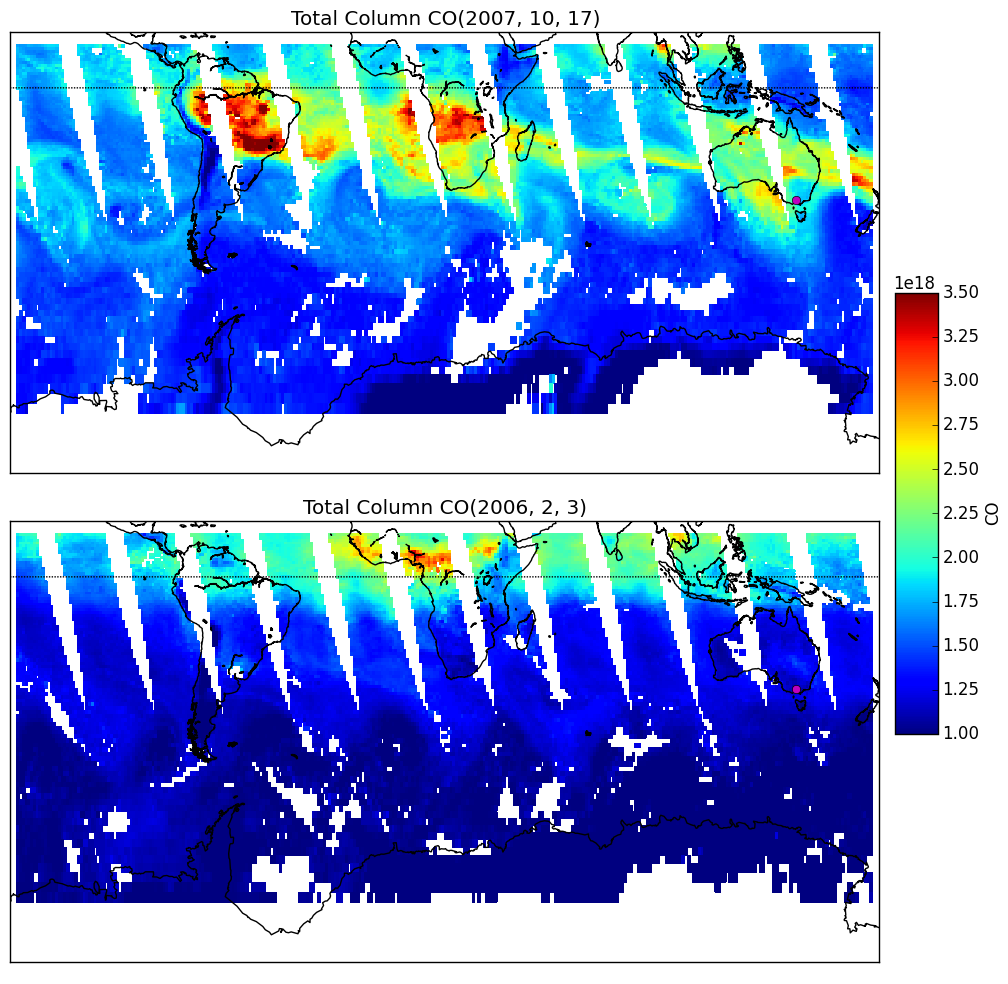
\includegraphics[width=\textwidth]{Figures/Ozone/AIRS_compare.png}
      \caption{AIRS total column CO image showing two days seperate days of swathes. The top panel shows an example of an excluded ozone event which could have been caused by a transported biomass burning plume on October 17th, 2007.}
      \label{ch_o3:fig:excludedeg}
    \end{figure}

  
\section{GEOS-Chem ozonesonde comparison}
  
  \subsection{GEOS-Chem UCX}
    TODO: Describe UCX run.
    
  \subsection{Determining tropospheric ozone from GEOS-Chem}
    GEOS-Chem allows certain diagnostics, along with any tracer, to be output at higher temporal resolution for a list of latitude and longitude based boxes.
    Storing output every six hours allows an examination of vertical profiles at a list of specific latitudes and longitudes during both day and night.
    Using the ozone mixing ratio ($C_{O_3}$ in molecules O$_3$ per molecule of air) at 72 vertical layers and the air density (N$_{Air}$ in molecules per cm$^3$), provides us with the ozone density profile (N$_{O_3}$):
    \begin{equation*}
     N_{O_3}[z] = C_{O_3}[z] \times N_{Air}[z]
    \end{equation*}
    where z is the vertical level index.
    
    In order the determine the tropospheric ozone column ($TC_{O_3}$ in molecules cm$^{-2}$), we first use the modelled tropopause pressure (TPP in hPa) to determine where the troposphere ends.
    The TPP is used to determine how many vertical levels exist in the troposphere.
    This is done through comparison with the pressure edges of each level.
    The linear fraction (frac) of the level containing the TPP is then obtained from the pressure edges below and above the TPP (pb and pa respectively):
    \begin{equation*}
     frac = \frac{p_b - TPP}{p_b-p_a}
    \end{equation*}
    
    At every time step, using the above calculations along with the layer heights (H in cm), the tropospheric ozone (TVC$_{O_3}$ in molecules cm$^{-2}$) is determined as follows: $N_{O_3}[z] \times H[z]$ gives the vertical profile of molecules cm$^{-2}$, which is then summed up to the TPP:
    \begin{equation*}
     TVC_{O_3} = \Sigma_{z=0}^{z_{TPP}-1} \left( N_{O_3}[z] \times H[z] \right) + frac \times N_{O_3}[z_{TPP}] \times H[z_{TPP}]
    \end{equation*}
    where $z_{TPP}$ is the index of the level containing the tropopause.
    
    Figure \ref{ch_o3:fig:StationSeriesGEOSChem} shows the time series of tropospheric ozone (TVC$_{O_3}$) simulated over our three stations from January 1 2005 to January 1 2011.
    Due to our simulation running with horizontal resolution of GEOS-Chem is 2$^{\circ}$ latitude by 2.5$^{\circ}$ longitude, and the profiles and totals above each site are actually the average over this horizontal area containing each station.
    All three sites have a discernable yearly cycle, with Davis having the least spread as well as the greatest outliers.
    These outlying tropospheric ozone columns all occur during the July to September months (TODO: reasons for why? simulated summer turbulence?).
    Both Macquarie Island and Melbourne have more variance in their tropospheric columns.
    For both sites the data is more spread out over the winter months.
    This variability is shown in more detail in figure \ref{ch_o3:fig:YearlyCyclGEOSChem}.
    
    Figure \ref{ch_o3:fig:YearlyCyclGEOSChem} shows the yearly averaged tropospheric ozone column over our three sites.
    This figure is created using the monthly averages along with their standard deviations.
    Melbourne has the largest tropical ozone column throughout the year, with a summer peak and winter minimum.
    Davis has the lowest ozone levels, with an opposite seasonal cycle to that of Melbourne.
    At Macquarie Island, there is a more subtle seasonal cycle, with slightly more ozone occuring in winter than in summer.
    
    \begin{figure}[!htbp]
      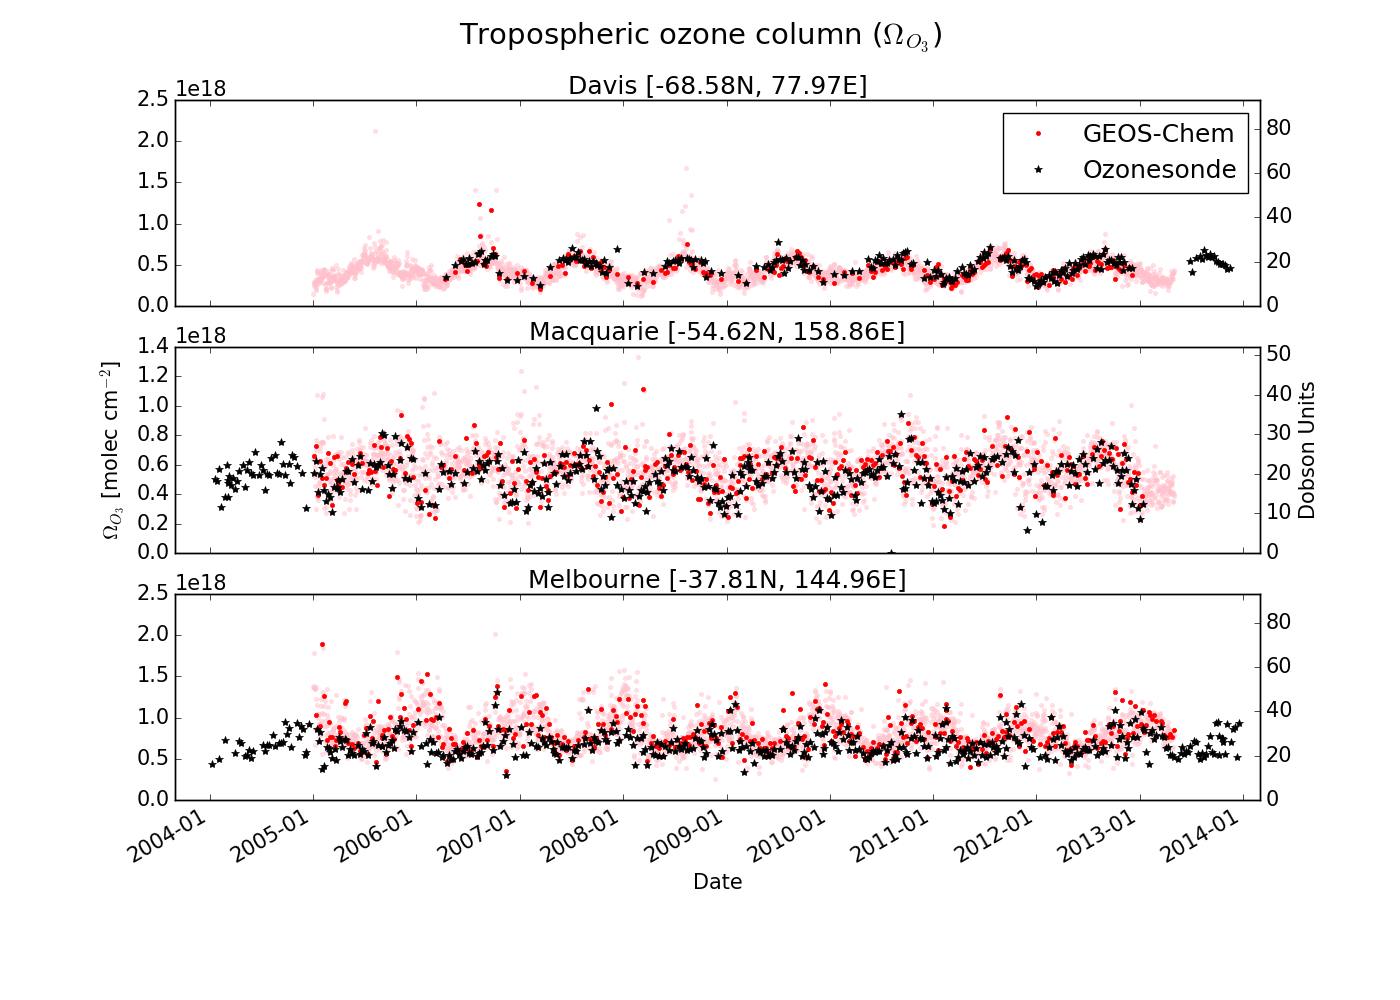
\includegraphics[width=\textwidth]{Figures/Ozone/StationSeries.png}
      \caption{Tropospheric ozone in molecules cm$^{-2}$ every six hours simulated by GEOS-Chem from January 1 2004 until December 31 2010. }
      \label{ch_o3:fig:StationSeriesGEOSChem}
    \end{figure}
    
    \begin{figure}[!htbp]
      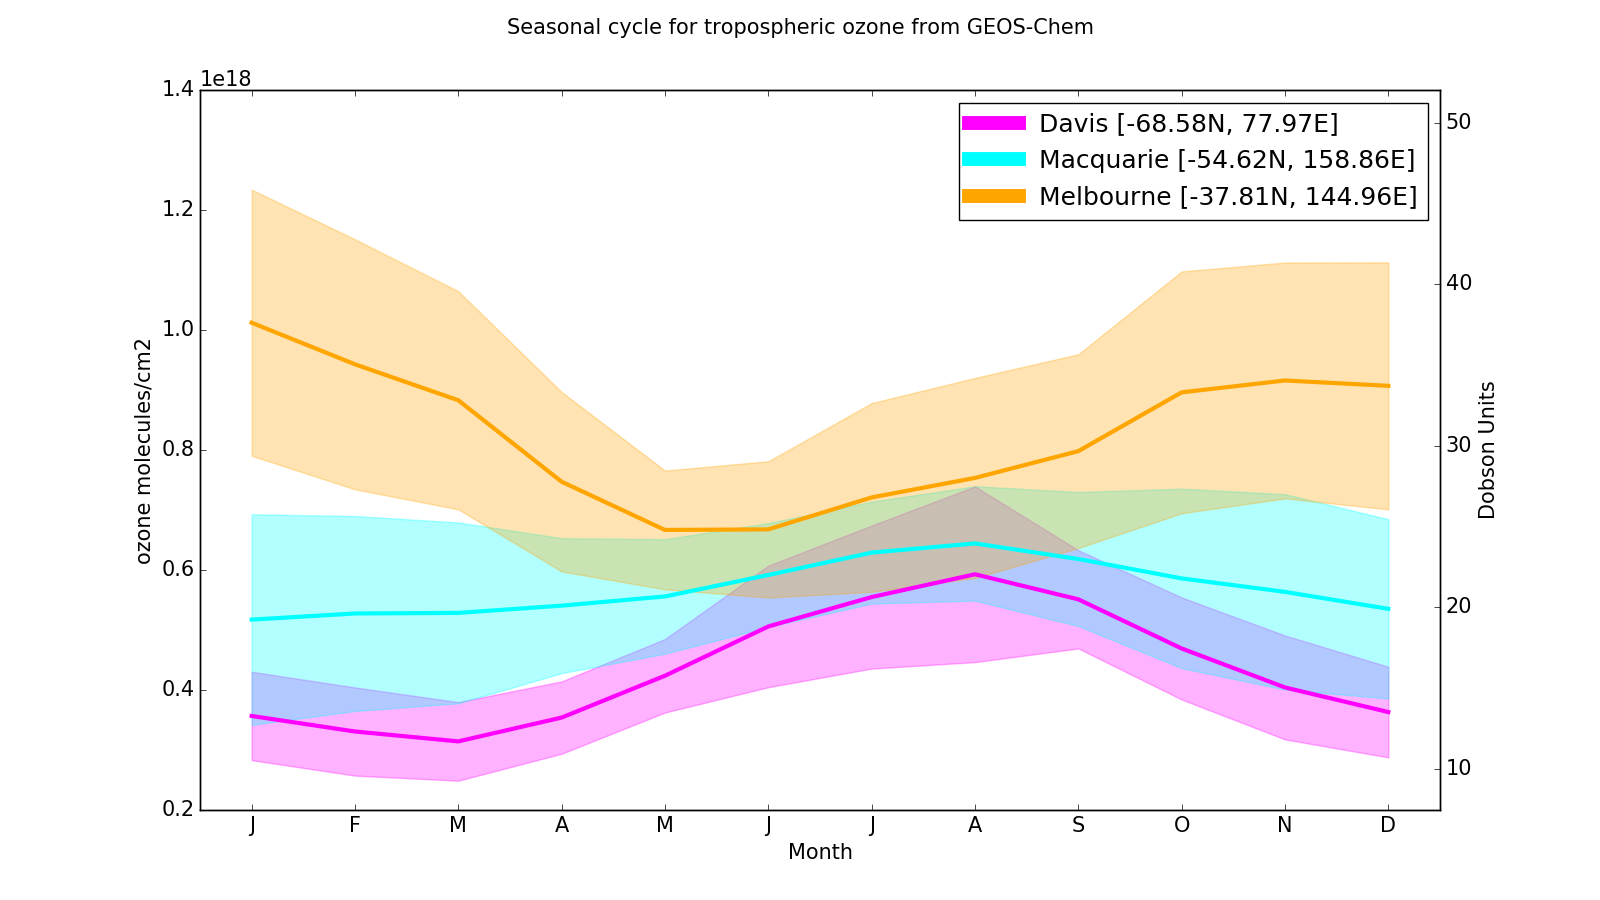
\includegraphics[width=\textwidth]{Figures/Ozone/Yearly_cycle.png}
      \caption{Tropospheric ozone in molecules cm$^{-2}$ seasonal cycle simulated by GEOS-Chem from January 1 2004 until December 31 2010. The monthly averages are taken for each year and the mean plotted with one standard deviation shaded.}
      \label{ch_o3:fig:YearlyCyclGEOSChem}
    \end{figure}
    
  \subsection{Profile from GEOS-Chem}
    GEOS-Chem provides 72 vertical levels of data, of which about 30 will be in the troposphere.
    Interpolating the vertical levels to a standard set of altitudes allows an examination of both the mean ozone profils and the standard deviation at each altitude.
    Recall that the profiles are output every 6 hours, so as well as getting the overall profile average it is easy to determine the daytime and night time average by only looking at particular hours.
    GEOS-Chem uses GMT/UTC time, outputting 4 profiles per day at 0~hrs, 6~hrs, 12~hrs, and 18~hrs.
    The local offset in time at Davis, Macquarie Island, and Melbourne is \+7~hrs, \+11~hrs, \+10~hrs respectively.
    
    Figures \ref{ch_o3:fig:GEOSChemMonthlyProfilesDavis}-\ref{ch_o3:fig:GEOSChemMonthlyProfilesMelbourne} show the monthly averaged ozone profile at Davis, Macquarie Island, and Melbourne respectively.
    The shaded areas show $\pm 1$ standard deviation, while the horizontal dotted line shows the mean tropopause height.
    The effect of pollution and mainland influence can be seen over Melbourne, mostly during the summer months (DJF), as the lower altitudes have increased ozone mean as well as more variance.
    Also the yearly cycle of tropopause height for each site is noticible, and it matches (TODO does it?) the ozonesonde recorded tropopause seasonal cycle.
    Examining the mean profiles at particular hours only shows a noticible difference (not shown unless someone tells me to) over Melbourne, the other two stations are very similar regardless of which hour we examine.
    
    \begin{figure}[!htbp]
      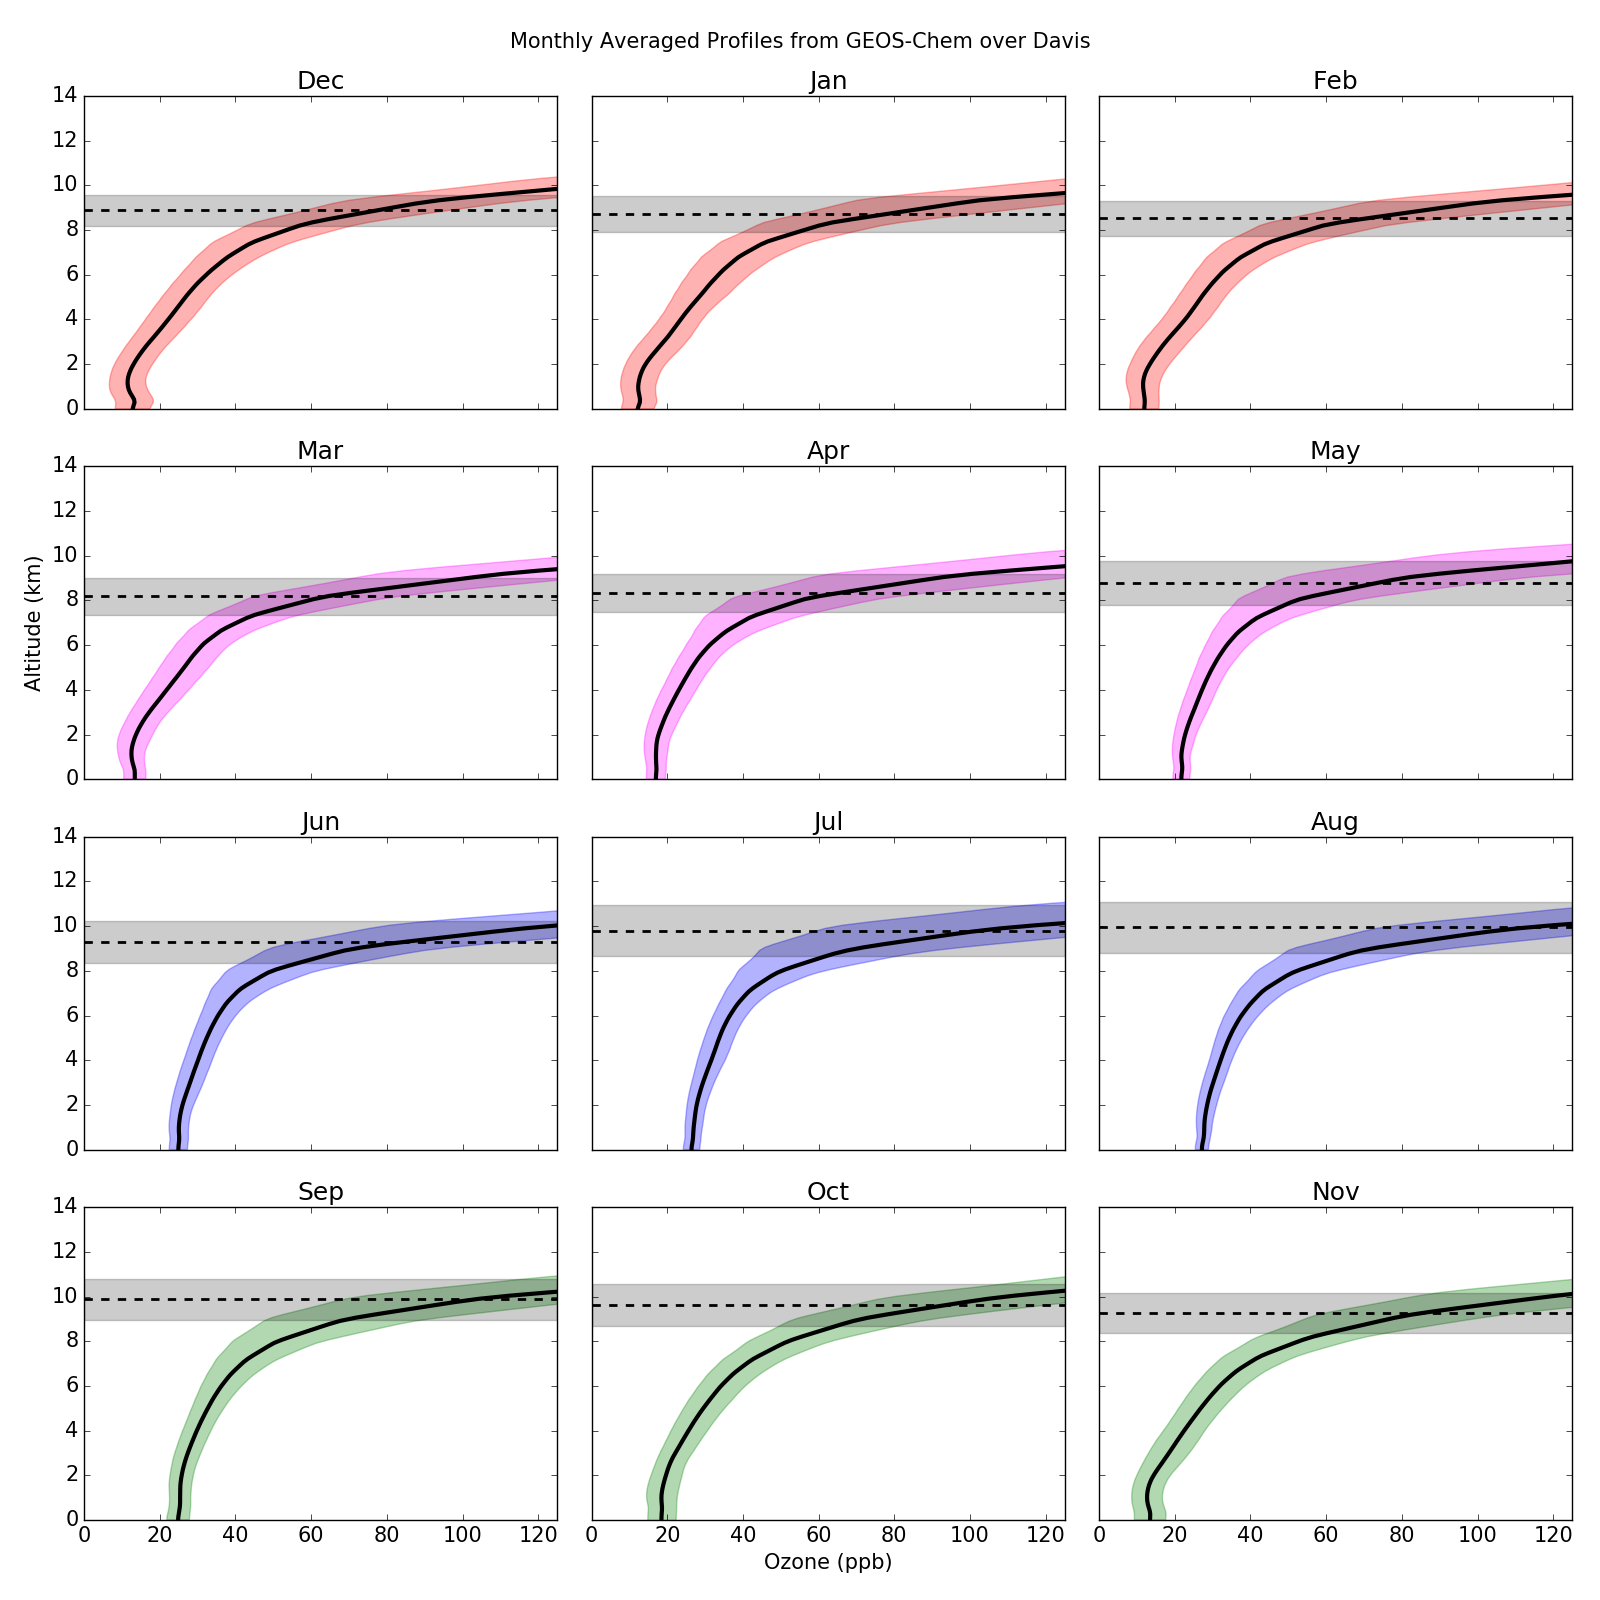
\includegraphics[width=\textwidth]{Figures/Ozone/Davis_profiles.png}
      \caption{Tropospheric ozone (ppb) simulated by GEOS-Chem over Davis from January 1 2004 until December 31 2010, averaged monthly.
      Shaded areas show one standard deviation, horizontal dotted line shows the mean tropopause height.}
      \label{ch_o3:fig:GEOSChemMonthlyProfilesDavis}
    \end{figure}
    \begin{figure}[!htbp]
      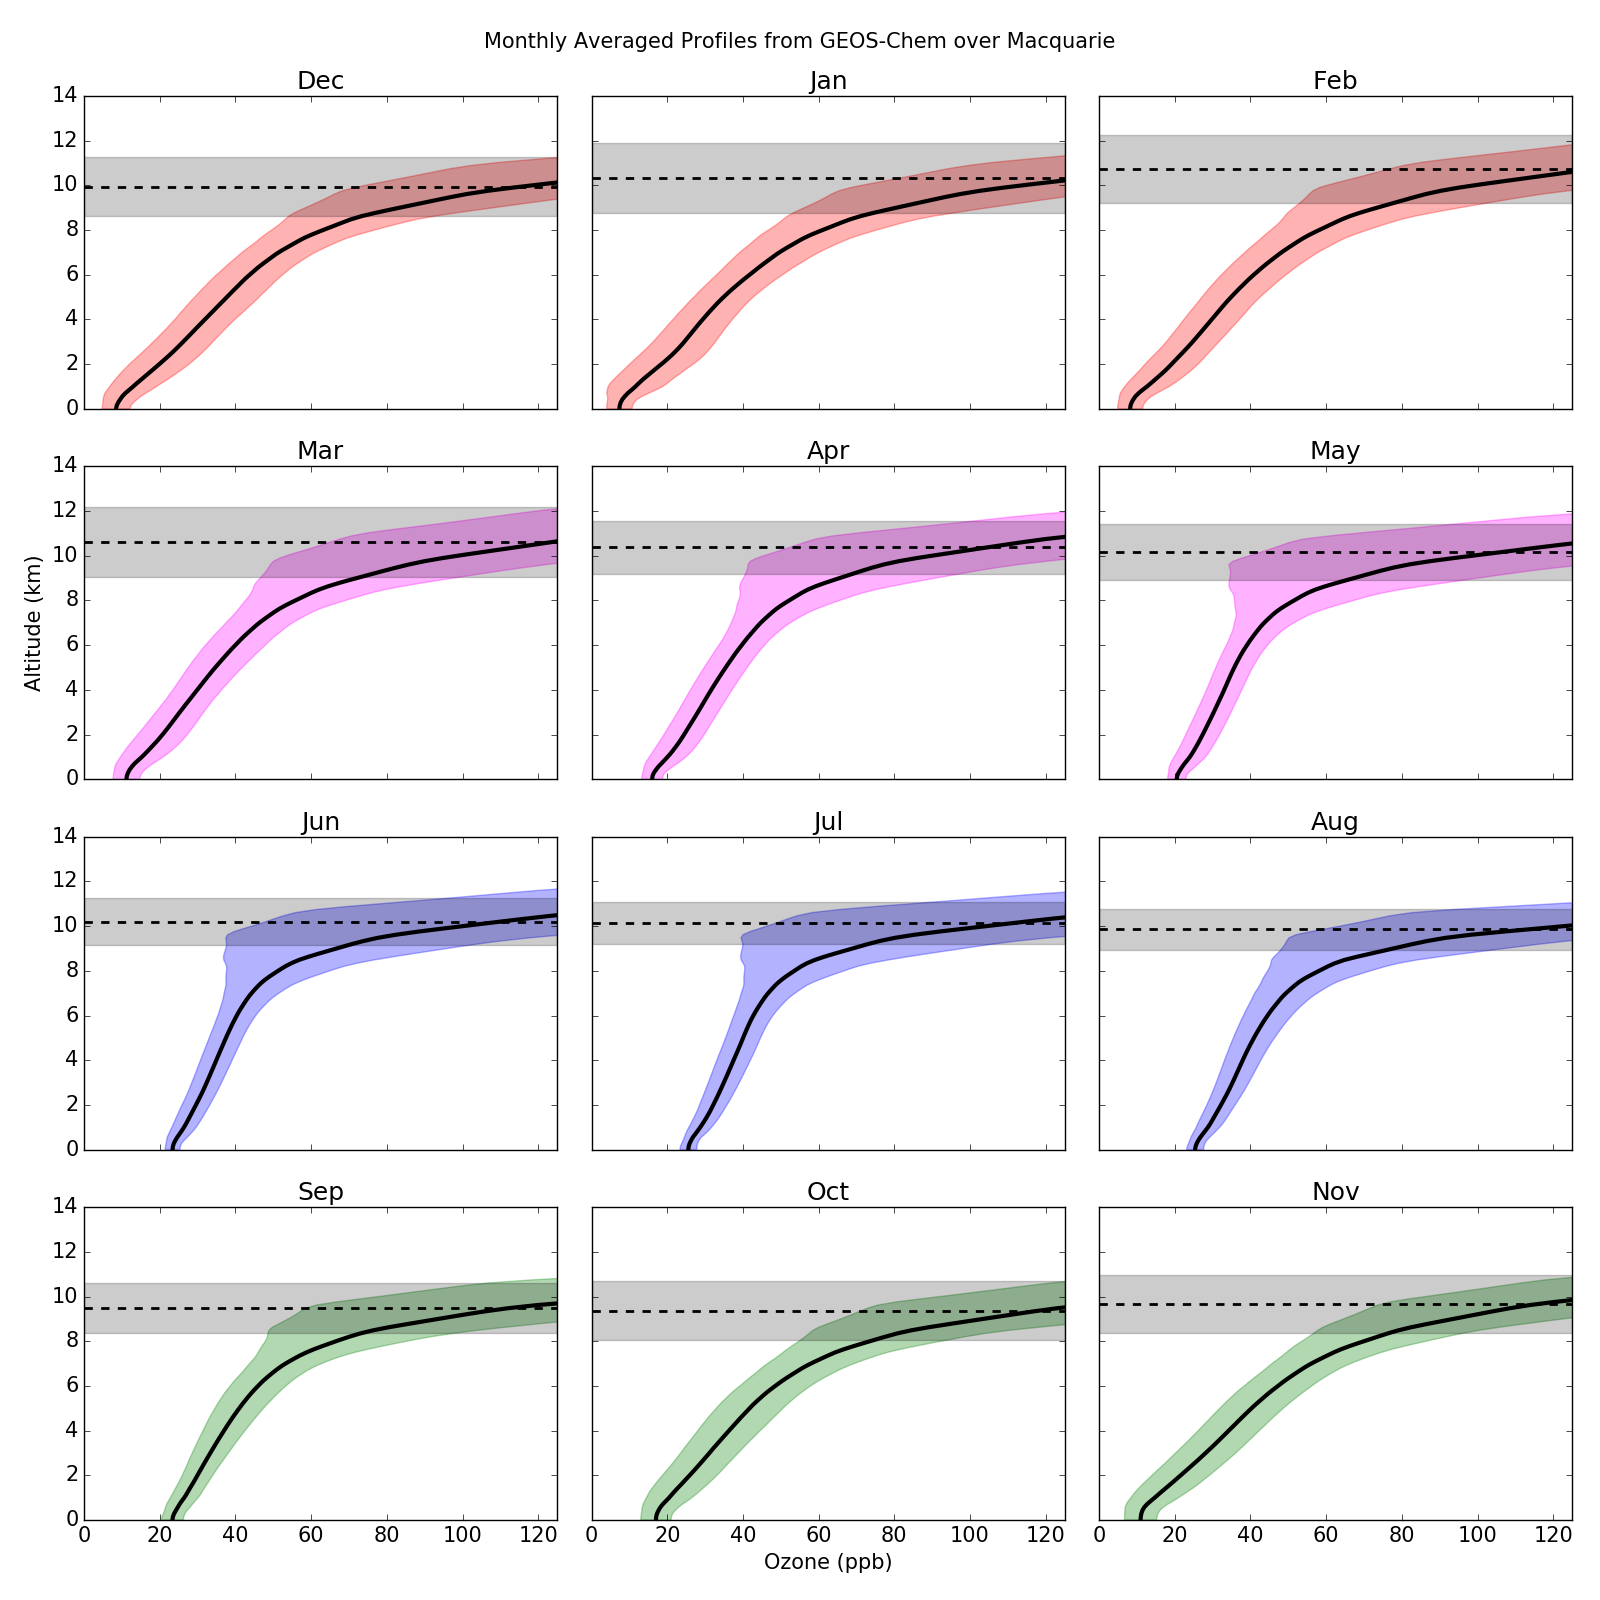
\includegraphics[width=\textwidth]{Figures/Ozone/Macquarie_profiles.png}
      \caption{As figure \ref{ch_o3:fig:GEOSChemMonthlyProfilesDavis} over Macquarie Island.}
      \label{ch_o3:fig:GEOSChemMonthlyProfilesMacquarie}
    \end{figure}
    \begin{figure}[!htbp]
      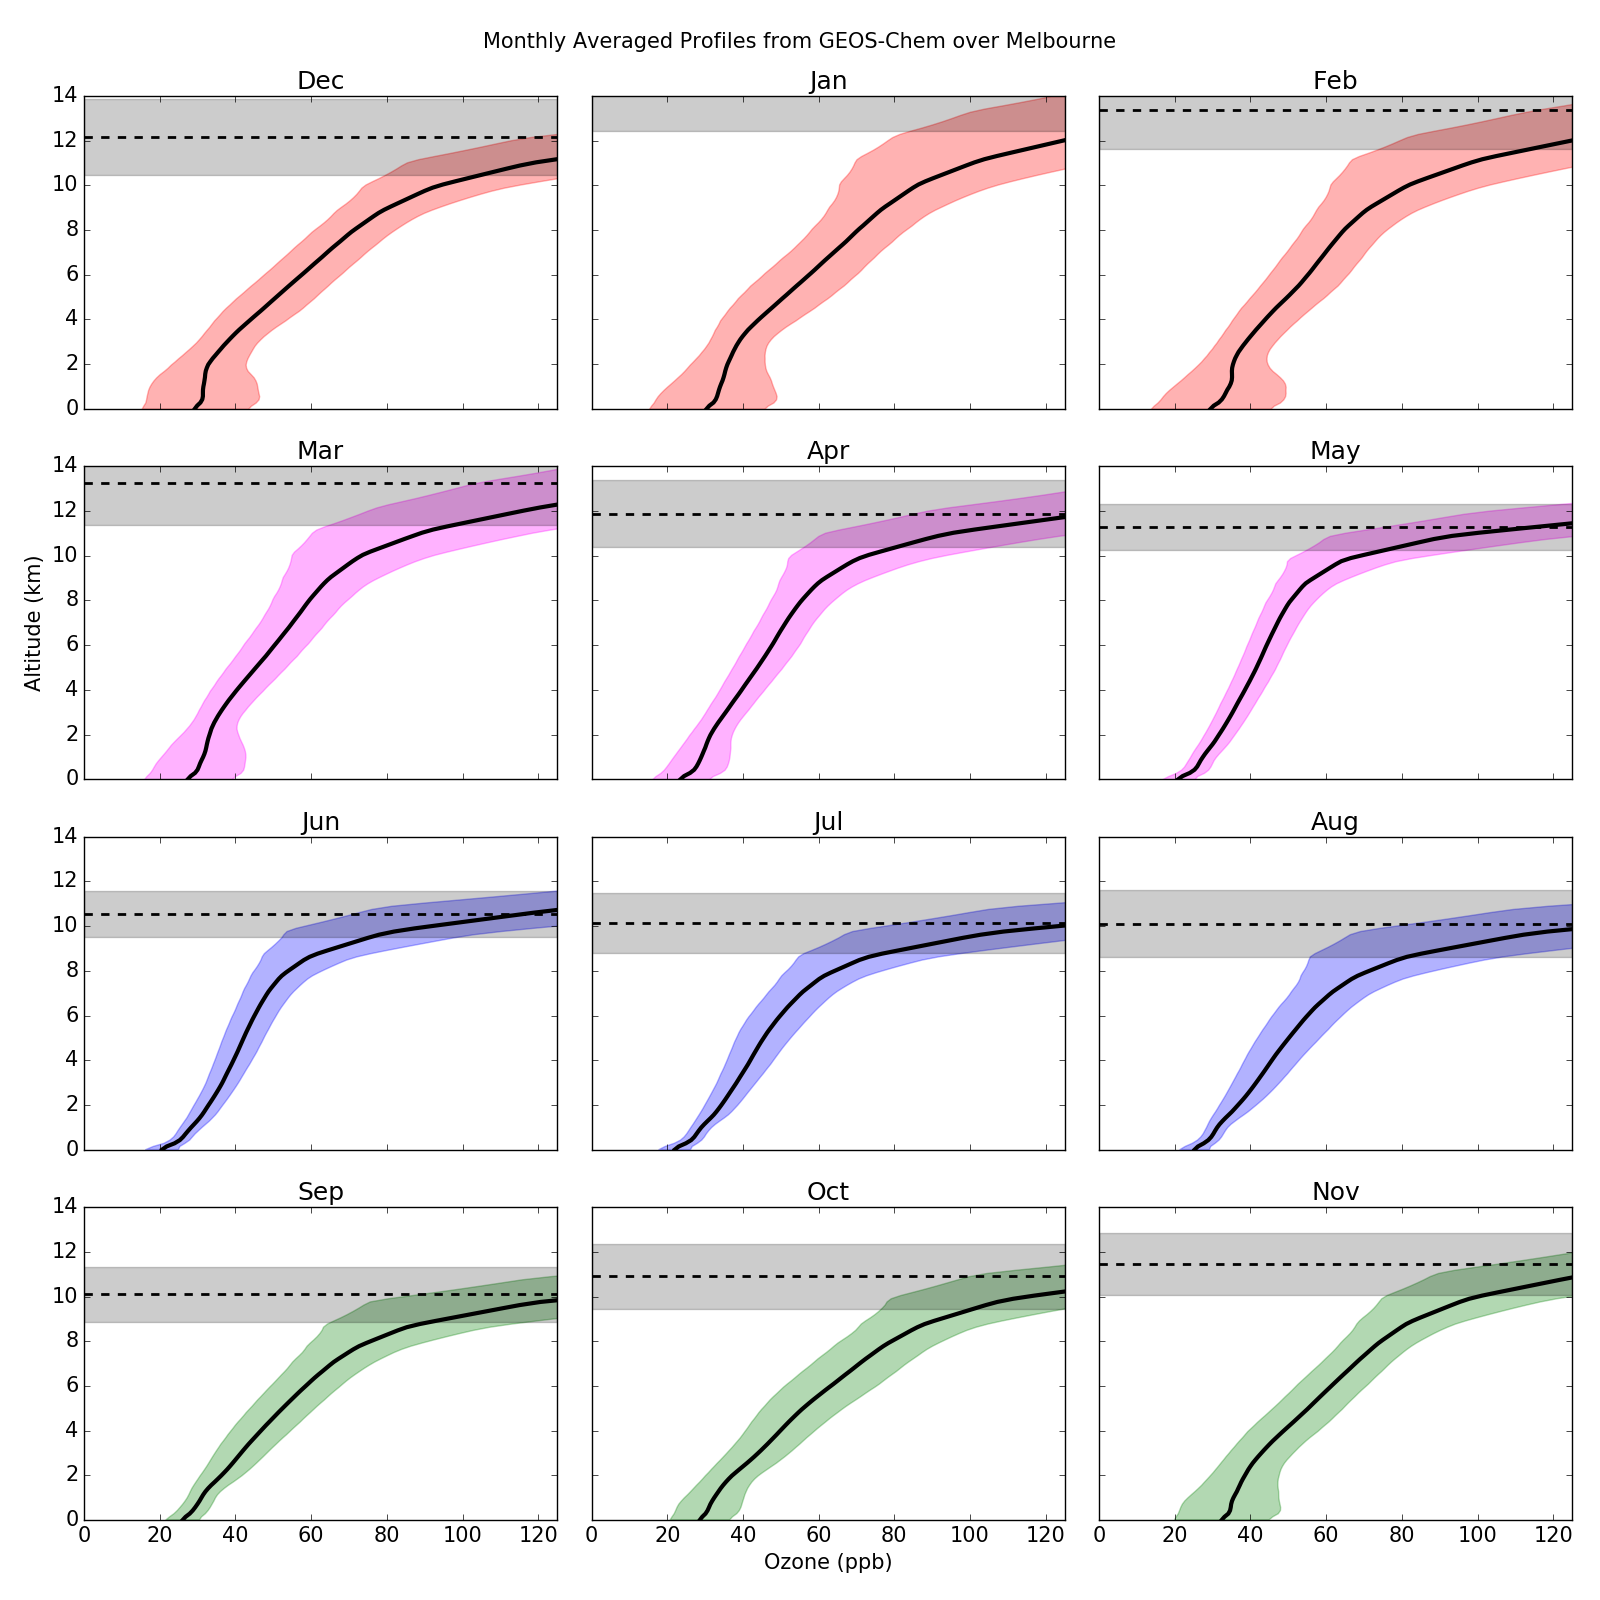
\includegraphics[width=\textwidth]{Figures/Ozone/Melbourne_profiles.png}
      \caption{As figure \ref{ch_o3:fig:GEOSChemMonthlyProfilesDavis} over Melbourne.}
      \label{ch_o3:fig:GEOSChemMonthlyProfilesMelbourne}
    \end{figure}
    
    TODO: Compare the mean profiles of ozonesonde events against the GEOS-Chem ones.

    Generally the vertical resolution of the GEOS-Chem ozone profile is too coarse to capture enough detail to determine whether or not an STT event is likely.
    Modelled Ozone profiles have roughly 30 levels below the tropopause, while the ozonesondes have upwards of 80.
    Figure TODO \ref{ch_o3:fig:GEOSChemEventProfilesSummary} shows the best and worst examples of the ozone profiles simulated and recorded above the three stations during detected STTs.
    These best and worst examples are determined qualitatively, and are shown as examples of the model-measurement differences.
    
    \begin{figure}[!htbp]
      \includegraphics[width=\textwidth]{Figures/Ozone/ModelledEventProfilesSummary.png}
      \caption{Simulated and recorded ozone profiles above Davis, Melbourne, and Macquarie Island respectively from top to bottom.
      The column on the left shows the best matching profile, while the right shows the worst (determined qualitatively).}
      \label{ch_o3:fig:GEOSChemEventProfilesSummary}
    \end{figure}
    
    Considering only the troposphere, I determine the correlation between the GEOS-Chem simulated profiles and the ozone sondes.
    In order to compare the tropospheric ozone ppb profile, first the ozonesonde recorded profiles are interpolated to match the vertical levels used by GEOS-Chem on the matching day.
    The interpolation takes the average of the recorded profile within each GEOS-Chem vertical level, and is referred to from here as the matched profile.
    This is done to remove any bias caused by the difference in simulated and recorded vertical resolution.
    The correlation is calculated by comparing the mean of the simulated and matched ozone profiles, up to the minimum of the tropopause altitudes determined through GEOS-Chem or from sondes.
    figure \ref{ch_o3:fig:GEOSChemTroposphereCorrelation} shows the correlation between mean modelled tropospheric ozone ppb.
    Quantitatively, the modelled tropospheric profile correlates well with the ozone sonde profiles.
    
    \begin{figure}[!htbp]
      \includegraphics[width=0.8\textwidth]{Figures/Ozone/GEOSChemTroposphericCorrelation.png}
      \caption{Correlation between the mean of simulated tropospheric ozone (ppb) and matched ozonesonde profiles (see text).}
      \label{ch_o3:fig:GEOSChemTroposphereCorrelation}
    \end{figure}
    
  \subsection{Estimation of southern ocean STT flux}
    
    